\chapter[Background]{Background}
\label{Chap:Background}

This chapter provides the required context for the topics discussed in this thesis. It covers the background knowledge for image processing, convolution, convolutional neural networks, compute platforms and the RISC-V ISA.

\section{Image Processing}
Image processing is the extraction of features from an image, to simplify it into a form that is more easily interpreted \cite{Mathworks}.
Generally, this refers to edge detection, object recognition, and image classification as parts of the processing pipeline.
Edge detection forms the basis of many image analysis techniques, as it is used to localize the variations in the image and to identify the physical phenomena which produce them.
These are classed as gradient-based or Laplacian based, though gradient-based algorithms are more widely used \cite{Gradient}.
The techniques do, however, share the commonality of being convolution-based, which requires a large number of multiplications and additions to compute.

The Robert, Prewitt and Sobel techniques are the most prominent of the gradient-based algorithms, applying convolution kernels to the image to detect edges \cite{Segmentation}.
\cite{XSG, Sobel, Canny, Aerial, Video} all provide a hardware implementation of the these filters, utilising the parallel processing capabilities of FPGAs to accelerate the gradient operations.
These designs realized improved efficiency in performance defined as increased throughput, and resource utilisation. 
Hence, FPGAs can provide a platform for processing real time algorithms on application-specific hardware with substantially higher performance than programmable digital signal processors (DSPs) \cite{RTEdge}.
This strongly indicates that FPGA-based implementations of image detection algorithms can offer significant improvements in running time for a range of digital signal processing methods, but were benchmarked only against microcontroller-based CPU platforms and not parallelised platforms.

The general pipeline for image detection and analysis is shown in Figure \ref{fig:pipeline}. 
This covers the available techniques which can be abstracted into hardware, to provide a high-speed, real-time image detection system.

\begin{figure}[h]
    \centering
    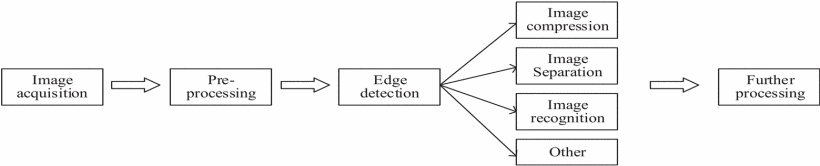
\includegraphics[width=1\textwidth]{Pipeline.png}
    \caption{Pipeline for image analysis techniques \cite{RTEdge}}
    \label{fig:pipeline}
\end{figure}

\cite{SoCImage, Aerial} follow a similar pipeline to Figure \ref{fig:pipeline}, with the image being captured by a camera module, and then processed by an FPGA though using differing image techniques.
These found that FPGAs can accelerate the required multiplication and addition operators separately - required for classical, and deep learning, based techniques \cite{ResourceEfficient}.
By leveraging the parallel processing capabilities of FPGAs to handle the convolution operations, the techniques can be accelerated to provide real-time image processing capabilities.

\section{Convolution}
Convolution operations form the computational foundation of many image processing and neural network applications.
It is referred to as a Single Instruction Multiple Data (SIMD) operation, as it performs the same operation on multiple data points in parallel \cite{7}.
In CNNs, convolution layers typically consume over 99\% of the total computational and storage resources \cite{18}.
Other sources estimate that convolution accounts for 90\% of the total execution time of CNNs, with between 50 to 90\% of the total operations being convolution \cite{3, 2}.
The operation involves sliding a kernel across input data, performing multiply-accumulate (MAC) operations between the kernel values and the input values at each position \cite{7}.
This process is depicted in Figure \ref{fig:convolution}.

\begin{figure}[h]
    \centering
    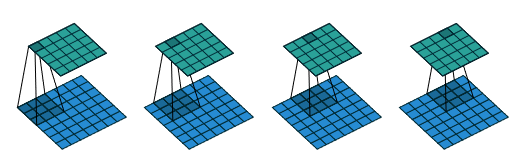
\includegraphics[width=1\textwidth]{Convolution.png}
    \caption{Convolution utilising a 3x3 kernel \cite{19}}
    \label{fig:convolution}
\end{figure}

For a single output pixel using an \(m \times n\) convolution mask, \(m \times n\) multiplications and \(m \times n-1\) additions are required. 
This computational intensity is demonstrated by the fact that processing a modest \(256 \times 256\) grayscale image with a \(3 \times 3\) mask requires \(589,824\) multiplications and \(65,535\) additions \cite{7}. 
The operation becomes even more resource-intensive when processing real-time video streams or larger images.
Hence, the convolution operation requires a large number of multiply-accumulate (MAC) operations, and is the primary bottleneck in the performance of CNNs \cite{11}.
The operation must window over the entire image, and the number of MAC operations is proportional to the size of the image and the number of filters in the layer.

Hardware implementations of convolution typically utilize one of two main approaches \cite{1}:
\begin{itemize}
    \item Direct computation using parallel processing units
    \item Data transformation methods, commonly used in frameworks like PyTorch and TensorFlow
\end{itemize}

FPGA implementations can significantly accelerate convolution operations through parallel processing. 
A common architecture involves storing image data and weights in block RAM (BRAM) \cite{7} or by embedding them in the FPGA fabric \cite{20} and implementing a finite state machine (FSM) to control pixel access and computation flow. 
Modern implementations often employ double-buffering techniques, where one buffer stores the working data while another handles intermediate results, enabling efficient pipelining of operations \cite{14}.

The pooling operation, which often follows convolution, operates similarly by sliding a window across the input but replaces the linear combination with alternative functions such as maximum or average calculations \cite{19}. 
Hence, it similarly shares the same hardware resources for adders and multipliers to compute.
This helps reduce the spatial dimensions of the data while retaining important features.

The number of operations, or hardware resources, required for convolution can be reduced through a number of optimization techniques. 
\begin{itemize}
    \item Quantisation to reduce precision requirements \cite{12}
    \item Sparsification to eliminate unused weights \cite{11}
    \item Time-division multiplexing (folding) of computing resources \cite{14}
    \item Streaming architectures that enable layer pipelining \cite{16}
\end{itemize}

These optimizations are particularly important for embedded systems and edge devices where computational resources and power consumption are constrained. 
For instance, quantization can reduce precision from 32-bit floating-point to 8-bit integer representations while maintaining accuracy within 0.1\% \cite{12}.
Other techniques can be used to compress the parameters to reduce the memory requirements \cite{18}.

\section{Convolutional Neural Networks}
Convolutional neural networks (CNNs) are a type of artificial neural network that is primarily used for image detection, as it uses the convolution kernel to detect features in the image.
Due to the lack of memory in low-end FPGA models, the CNN is optimal for an image processing task on SoC, as it has a low number of weights and biases relative to other neural networks \cite{Drowsiness}.
This makes it viable to implement machine learning cores through a CNN using on-board resources with some optimisations compared to other more storage-intensive networks \cite{14}.

Similar works for image-analysis using different neural network architectures have also been implemented using FPGA hardware.
\cite{Yolo, SparseYolo} demonstrates a hardware implementation of the You Only Look Once (YOLO) algorithm using a Xilinx Virtex-7 FPGA. 
Like the CNN hardware implementations, the architecture is focused on accelerating the convolution operation - and is a common denominator in the performance neural networks in hardware.
This acceleration is not specific to the convolution operator, and can be applied to any intensive operation in the network as the FPGA has little overhead on each operator when compared to traditional platforms \cite{Overhead}.
This is corroborated by \cite{Throughput}, which found that the implementation of hybrid neural networks on a Xilinix Virtex-7 690T FPGA achieved 4.13 times higher throughput than state of the art accelerators in 2019.


\section{RISC-V}
Instruction set architectures (ISAs) define the operations a processor can execute, however, the majority of ISAs are proprietary and require licensing to use.
Reduced Instruction Set Computing (RISC) is a form of ISA which offers a simpler, more efficient design than the traditional Complex Instruction Set Computing (CISC) ISAs - such as the prevalent x86 instruction set \cite{Arm}.
Arm and RISC-V are the two most prominent RISC ISAs, with Arm being the most widely used in embedded systems but with RISC-V offering royalty-free licensing and an open-source nature.
The lack of licensing fees and the open-source nature of RISC-V has led to its increasing popularity in the embedded systems domain \cite{Neutron}.
It is estimated that the number of chips utilising RISC-V technology "will grow 73.6 percent per year to 2027, when there will be some 25 billion AI chips produced, accounting for US \$291 billion in revenue" \cite{Drowsiness}.


There exists a number of FPGA implementations to create softcore processors using the RISC-V ISA \cite{RISCFPGA}. 
This 2023 paper \cite{Neutron} demonstrates a RISC-V implementation of the NEORV32 core, using a Wishbone bus interface. 
The authors selected the NEORV32 core due to it being vendor-agnostic and platform independent, with the project being highly documented.
The softcore nature allows for the implementation details to be customised to the specific application, such that the core can be adapted to the specific use case \cite{DCT}. 
The NEORV32 processors offers a system-on-chip (SoC) Harvard architecture, with a 32-bit RISC-V processor, and a range of peripherals.
It supports UART, SPI, standard GPIO and the Wishbone b4 external bus interface for SoC connectivity \cite{NEORV32}.

As it is an open-source ISA, RISC-V has the added benefit of being extensible and modular \cite{Cryptography}, allowing for instructions to be added to the processor.
\cite{Reconfigurable} utilises this to create custom instructions within the RISC-V ISA to accelerate the expensive convolution operation for a CNN.
Other applications have also extended the architecture to include custom instructions for frequently used and computationally-expensive operations.

\section{Computing Platforms}
\label{sec:platforms}
The nature of convolution, and many of the layers in CNNs, benefit significantly from parallel processing capabilities.

Field Programmable Gate Arrays (FPGAs) provide flexible compute resources that can be reconfigured to suit a wide range of applications. Similar to graphics processing units (GPUs), FPGAs offer parallel processing capabilities, but with the added benefit of reconfigurability \cite{Parallelism}. The ability to develop custom logic designs is not unique to FPGAs, as application-specific integrated circuits (ASICs) also offer this capability. ASICs offer better optimization in many aspects than FPGAs, but cannot be reconfigured and require a large upfront cost for design and fabrication \cite{AsicOptimization}. This makes FPGAs a more suitable platform for low-volume production and prototyping, as they offer a faster development cycle and lower cost than ASICs.

In contrast, traditional Central Processing Units (CPUs) are designed for serial processing, executing a single instruction stream at a time - see figure \ref{fig:cpu_gpu}. This architecture is optimized for low-latency tasks and complex control logic, making CPUs highly effective for general-purpose computing. However, their performance can be limited when handling tasks that require high levels of parallelism, such as those found in image processing and deep learning applications. 
On the other hand, GPUs are specifically designed for parallel processing, featuring thousands of cores that can execute multiple threads simultaneously. 
This architecture allows GPUs to handle large datasets and perform computations in parallel, significantly speeding up tasks like matrix multiplications and convolutions, which are fundamental in CNNs \cite{15}.
The parallel architecture can be implemented in FPGA fabric, to achieve drastic speedups.
\cite{10} demonstrates a twenty-times speedup of the throughput when the network was compared to a CPU implementation, similar or better results would be expected for a GPU implementation.

The CUDA (Compute Unified Device Architecture) platform, developed by NVIDIA, further enhances the capabilities of GPUs by providing a parallel computing framework that allows developers to leverage the power of GPU cores, known as CUDA cores. Each CUDA core is capable of executing a thread, and with thousands of these cores available, GPUs can perform massive parallel computations efficiently \cite{4}. This makes CUDA particularly well-suited for applications in machine learning, where the ability to process large amounts of data simultaneously is crucial \cite{22}. 

NVIDIA's GPUs are designed with a focus on high throughput and efficiency, making them ideal for tasks that require extensive computational power. The architecture of NVIDIA GPUs includes multiple Streaming Multiprocessors (SMs), each containing several CUDA cores \cite{4}. This design allows for the simultaneous execution of thousands of threads, enabling the GPU to handle complex calculations much faster than a CPU. For instance, while a CPU may have a few cores optimized for sequential processing, a modern NVIDIA GPU can have thousands of CUDA cores working in parallel, which is particularly beneficial for deep learning tasks that involve large matrices and tensors.

The combination of GPU architecture and the CUDA platform has led to significant advancements in the performance of deep learning algorithms, enabling real-time processing and analysis of complex datasets. 
For example, in image recognition tasks, the parallel processing capabilities of GPUs allow for the rapid analysis of thousands of images simultaneously, which is essential for training deep neural networks effectively \cite{16}.

These reconfigurable platforms are optimal for edge applications on images, due to the parallelized pipeline structure, which enables high-speed processing of large amounts of image data, and their high processing speed ensures real-time image data processing \cite{Video}. FPGAs in particular have been studied extensively in the field of image detection, as replacements for existing hardware infrastructures due to the increasing complexity of algorithms \cite{ResearchFPGA}. They offer low latency and low power consumption due to their computing characteristics. However, the ability to configure often means that resource constraints and utilization must be considered when designing the system, such as with many embedded devices.

\begin{figure}[h]
    \centering
    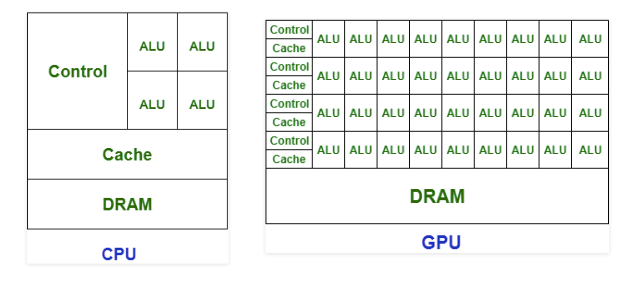
\includegraphics[width=0.8\textwidth]{cpu.png}
    \caption{Comparison of logic units between CPU and GPU \cite{21}}
    \label{fig:cpu_gpu}
\end{figure}